\section{Performance Regression Analysis}
\label{src:regression}
Creating multiple symmetric memory partitions would result in
multiple symmetric heaps on each PE. The symmetric heap maintenance
includes memory registration with NIC and offset maintenance on
each PE. Though upcoming communication layers like
libfabrics~\cite{libfabrics} have support for Scalable memory
Registration, Cray SHMEM implementation over DMAPP uses basic memory
registration and hence there is a increase in memory footprint on
DMAPP-level on maintaining symmetric heaps on each PE.

\vspace{-20pt}
\begin{algorithm}[!h]
\begin{algorithmic}
    \Procedure{\texttt{shmem\_putmem}}
    {void *dest, const void *src, size\_t nblks, int pe\_id}\;
        dmapp\_seg\_desc\_t *target\_seg = \texttt{NULL}\;
        dmapp\_type\_t type = \texttt{DMAPP\_BYTE}\;
        \If {\normalfont (dest.segment $\equiv$
                         \texttt{DATA\_SEGMENT})} {
            target\_seg = \texttt{DATA\_SEGMENT}\;
        } \ElseIf {\normalfont (dest.segment $\equiv$
                         \texttt{SHEAP\_SEGMENT})} {
            target\_seg = \texttt{SHEAP\_SEGMENT}\;
        } \Else {
            segment\_identified = \textit{false}\;
            \For {\normalfont (int i = 1; i $\leq$ N; i++)}{
                \If{\normalfont (dest.segment $\equiv$
                    \texttt{USER\_SEGMENT\_i})} {
                    target\_seg = \texttt{USER\_SEGMENT\_i})\;
                    segment\_identified = \textit{true}\;
                }
            }
            \If{\normalfont(segment\_identified $\equiv$
                    \textit{false})} {
                abort()\;
            }
        }
        dmapp\_put(dest, target\_seg, pe\_id, src, nelems, type)\;
        return\;
    \EndProcedure
    \caption{Lookup logic with N symmetric memory partitions per PE}
    \label{algo:normal-lookup}
\end{algorithmic}
\end{algorithm}
\vspace{-20pt}

Apart from the increase in memory footprint on memory registration,
identifing the correct symmetric heap segment before performing an
underlying communication operation is essential. %with symmetric heap lookup on each
%RMA and AMO operation is expected to introduce performance
%regression.
Algorithm~\ref{algo:normal-lookup} shows the introduction lookup
logic trying to match the correct symmetric heap segment on the
\texttt{shmem\_putmem} operation. Similar, lookups are introduced in
all OpenSHMEM RMA and AMO operations. \texttt{USER\_SEGMENT} refers to
the symmetric heap segments created on user-defined memory partitions.

\begin{figure*}[h!]
    \vspace{-30pt}
    \centering
    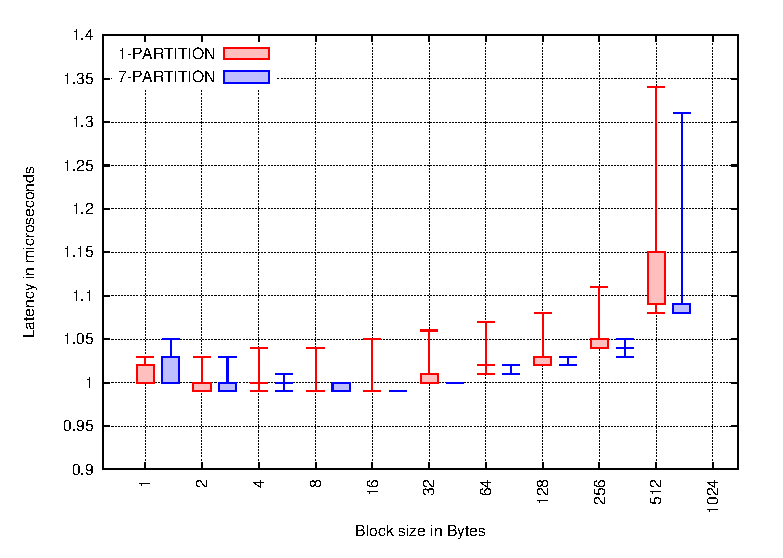
\includegraphics[width=\linewidth]{graph/osu-put.eps}
    \caption{Performance difference on using destination buffers
    from 1 partition and 7 partitions
    on modified OSU Put microbenchmark}
    \label{graph:lookup}
    \vspace{-20pt}
\end{figure*}

We measured the performance regression behind this additional lookup
operation using a modified OSU microbenchmark~\cite{pgas-benchmarks}
on a Cray XC system with Intel KNL processors. We used 2 PEs with 1
PE per node for the tests.
The normal OSU microbenchmark selects the buffer from the memory
segment (either \texttt{DATA\_SEGMENT} or \texttt{SHEAP\_SEGMENT})
per job. We modified the \texttt{shmem\_putmem} benchmark by creating
one destination buffer per \texttt{N} partitions and randomly select
the destination buffer from different partitions for every iteration.
We timed the average performance of all the iterations of the
\texttt{shmem\_putmem} operation.

Figure~\ref{graph:lookup} shows the
performance difference between using 1 and 7 partitions on very small
data sizes. The average performance variations is around 2\% to
3\% and this can be attributed as noise. But, if we increase
the number of partitions to 127, we could see the variation as high
as 6\%. We expect users to create only one partition per memory kind
and not \texttt{N} unnecessary partitions. Moreover, as mentioned in
Table~\ref{tab:const} the \texttt{SHMEMX\_MAX\_PARTITIONS} library
constant in Cray SHMEM is 7.

We observe similar performance variation on small data sizes on other
RMA and AMO operations. For larger message sizes, the segment lookup
does not contribute much for any performance variation.

\section{Performance Analysis}
\label{src:perf}